\documentclass[hyperref, a4paper]{article}

\usepackage{geometry}
\usepackage{titling}
\usepackage{titlesec}
% No longer needed, since we will use enumitem package
% \usepackage{paralist}
\usepackage{enumitem}
\usepackage{footnote}
\usepackage[colorinlistoftodos]{todonotes}
\usepackage{amsmath, amssymb, amsthm}
\usepackage{mathtools}
\usepackage{bbm}
\usepackage{graphicx}
\usepackage{subcaption}
\usepackage{soulutf8}
\usepackage{physics}
\usepackage{tensor}
\usepackage{siunitx}
\usepackage[version=4]{mhchem}
\usepackage{tikz}
\usepackage{xcolor}
\usepackage{listings}
\usepackage{autobreak}
\usepackage[ruled, vlined, linesnumbered]{algorithm2e}
\usepackage{acro}
\usepackage{nameref,zref-xr}
\zxrsetup{toltxlabel}
\usepackage[backend=bibtex,sorting=none]{biblatex}
\addbibresource{floquet.bib}
\usepackage[colorlinks,unicode]{hyperref} % , linkcolor=black, anchorcolor=black, citecolor=black, urlcolor=black, filecolor=black
\usepackage[most]{tcolorbox}
\usepackage{prettyref}

% Page style
\geometry{left=3.18cm,right=3.18cm,top=2.54cm,bottom=2.54cm}
\titlespacing{\paragraph}{0pt}{1pt}{10pt}[20pt]
\setlength{\droptitle}{-5em}

% More compact lists 
\setlist[itemize]{
    itemindent=17pt, 
    leftmargin=1pt,
    listparindent=\parindent,
    parsep=0pt,
}

% Math operators
\DeclareMathOperator{\timeorder}{\mathcal{T}}
\DeclareMathOperator{\diag}{diag}
\DeclareMathOperator{\legpoly}{P}
\DeclareMathOperator{\primevalue}{P}
\DeclareMathOperator{\sgn}{sgn}
\DeclareMathOperator{\res}{Res}
\newcommand*{\ii}{\mathrm{i}}
\newcommand*{\ee}{\mathrm{e}}
\newcommand*{\const}{\mathrm{const}}
\newcommand*{\suchthat}{\quad \text{s.t.} \quad}
\newcommand*{\argmin}{\arg\min}
\newcommand*{\argmax}{\arg\max}
\newcommand*{\normalorder}[1]{: #1 :}
\newcommand*{\pair}[1]{\langle #1 \rangle}
\newcommand*{\fd}[1]{\mathcal{D} #1}
\DeclareMathOperator{\bigO}{\mathcal{O}}

% TikZ setting
\usetikzlibrary{arrows,shapes,positioning}
\usetikzlibrary{arrows.meta}
\usetikzlibrary{decorations.markings}
\usetikzlibrary{calc}
\tikzstyle arrowstyle=[scale=1]
\tikzstyle directed=[postaction={decorate,decoration={markings,
    mark=at position .5 with {\arrow[arrowstyle]{stealth}}}}]
\tikzstyle ray=[directed, thick]
\tikzstyle dot=[anchor=base,fill,circle,inner sep=1pt]

% Algorithm setting
% Julia-style code
\SetKwIF{If}{ElseIf}{Else}{if}{}{elseif}{else}{end}
\SetKwFor{For}{for}{}{end}
\SetKwFor{While}{while}{}{end}
\SetKwProg{Function}{function}{}{end}
\SetArgSty{textnormal}

\newcommand*{\concept}[1]{{\textbf{#1}}}

% Embedded codes
\lstset{basicstyle=\ttfamily,
  showstringspaces=false,
  commentstyle=\color{gray},
  keywordstyle=\color{blue}
}

% Reference formatting
\newcommand*{\citesec}[1]{\S~{#1}}
\newcommand*{\citechap}[1]{chap.~{#1}}
\newcommand*{\citefig}[1]{Fig.~{#1}}
\newcommand*{\citetable}[1]{Table~{#1}}
\newcommand*{\citepage}[1]{pp.~{#1}}
\newrefformat{fig}{Fig.~\ref{#1}}
\newcommand*{\term}[1]{\textit{#1}}

% Color boxes
\tcbuselibrary{skins, breakable, theorems}

\newtcbtheorem{infobox}{Box}{
    enhanced,
    boxrule=0pt,
    colback=blue!5,
    colframe=blue!5,
    coltitle=blue!50,
    borderline west={4pt}{0pt}{blue!65},
    sharp corners,
    fonttitle=\bfseries, 
    breakable,
    before upper={\parindent15pt\noindent}}{box}
\newtcbtheorem[use counter from=infobox]{theorybox}{Box}{
    enhanced,
    boxrule=0pt,
    colback=orange!5, 
    colframe=orange!5, 
    coltitle=orange!50,
    borderline west={4pt}{0pt}{orange!65},
    sharp corners,
    fonttitle=\bfseries, 
    breakable,
    before upper={\parindent15pt\noindent}}{box}
\newtcbtheorem[use counter from=infobox]{learnbox}{Box}{
    enhanced,
    boxrule=0pt,
    colback=green!5,
    colframe=green!5,
    coltitle=green!50,
    borderline west={4pt}{0pt}{green!65},
    sharp corners,
    fonttitle=\bfseries, 
    breakable,
    before upper={\parindent15pt\noindent}}{box}


\newenvironment{shelldisplay}{\begin{lstlisting}}{\end{lstlisting}}

% Shorthands
\DeclareAcronym{arpes}{long = angle-resolved photoemission spectroscopy, short = ARPES}

\newcommand*{\kB}{k_{\text{B}}}
\newcommand*{\muB}{\mu_{\text{B}}}
\newcommand*{\efermi}{E_{\text{F}}}
\newcommand*{\pfermi}{p_{\text{F}}}
\newcommand*{\vfermi}{v_{\text{F}}}
\newcommand*{\sA}{\text{A}}
\newcommand*{\sB}{\text{B}}
\newcommand*{\Tc}{T_{\text{c}}}
\newcommand*{\hethree}{$^3$He}
\newcommand*{\hefour}{$^4$He}
\newcommand{\epsr}{\epsilon_{\text{r}}}
\newcommand{\chie}{\chi_{\text{e}}}
\newcommand{\Efreq}{\tilde{\vb{E}}}
\newcommand{\Dfreq}{\tilde{\vb{D}}}
\newcommand{\Pfreq}{\tilde{\vb{P}}}

\newcommand*{\Gammae}{\Gamma_{\text{e}}}
\newcommand*{\Gammag}{\Gamma_{\text{g}}}
\newcommand*{\omegae}{\omega_{\text{e}}}
\newcommand*{\omegag}{\omega_{\text{g}}}
\newcommand*{\omegaeg}{\omega_{\text{eg}}}
\newcommand*{\ptwfc}[2]{\psi^{(#2)}_{#1}}
\newcommand*{\mueg}{\mu_{\text{eg}}}
\newcommand*{\muge}{\mu_{\text{ge}}}
\newcommand*{\Ezzero}{E_{z0}}
\newcommand*{\kete}{\ket*{\text{e}}}
\newcommand*{\ketg}{\ket*{\text{g}}}
\newcommand*{\coeffe}{c_{\text{e}}}
\newcommand*{\coeffg}{c_{\text{g}}}
\newcommand*{\pope}{p_{\text{e}}}
\newcommand*{\popg}{p_{\text{g}}}

\title{Floquet theory}
\author{Jinyuan Wu}

\begin{document}

\maketitle

\section{Introduction} 

\section{The Floquet formalism: quasienergies and quasi-stationary states}

% Why we are able to do time-dependent projection 
% is not one hundred percent clear; 
% it's kind of like a constraint problem in classical mechanics:
% we already know a little about what will happen  
% (the state of EM doesn't change; the particle is confined on the plane, etc.)
% instead of what factors are small, 
% and we want to build an effective theory on top of that knowledge.
In this section we outline the basic formalism of Floquet physics,
following the notation in \cite{rudner2020floquet}.
As is mentioned in the introduction,
Floquet effects happen with a time-periodic Hamiltonian;
below we let $T = 2 \pi / \omega$ be the period.
Such a Hamiltonian is usually an effective Hamiltonian
when the system (hereafter ``matter'')
is coupled with another degree of freedom
which does not change much in the time evolution;
the latter is hereafter called ``light'',
since in condensed matter systems, 
periodic driving is usually achieved by 
shedding a beam of light to the matter:
consider the general form of light-matter interaction Hamiltonian 
with only one active photon mode
\begin{equation}
    H_{\text{full}} = 
    H \otimes 1_{\text{light}} +     
    \underbrace{
        1_{\text{matter}} \otimes \hbar \omega \left(
        b^\dagger b + \frac{1}{2} 
        \right) 
    }_{H_{\text{light}}}
    + \underbrace{
        b V + b^\dagger V^\dagger  
    }_{H_{\text{light-matter coupling}}} ,
    \label{eq:full-light-matter}
\end{equation}
and we assume that the state of the electromagnetic part 
is close to a coherent state $\ket*{\alpha \ee^{- \ii \omega t}}$ 
with strong intensity that almost has zero time evolution. 
Under this assumption, we can project out the electromagnetic degree of freedom by 
\begin{equation}
    P = \sum_{i} \ket*{i} \bra*{i} \otimes \bra*{\alpha \ee^{- \ii \omega t}}, 
    \label{eq:from-extended-to-matter}
\end{equation} 
where $i$ labels eigenstates of the matter degrees of freedom,
and this means the Hamiltonian for the matter part is 
\begin{equation}
    H_{\text{driven}} = P H_{\text{full}} P^\dagger - \ii \hbar P \partial_t P^\dagger = 
    H + \alpha V \ee^{- \ii \omega t} + \alpha^* V^\dagger \ee^{\ii \omega t},
    \label{eq:h-eff-matter}
\end{equation}
since 
\[
    P H_{\text{light}} P^\dagger = \hbar \omega \left(\abs*{\alpha}^2 + \frac{1}{2}\right), 
\]
and 
\[
    - \ii \hbar P \partial_t P = - \sum_i \dyad{i} \otimes \bra*{\alpha \ee^{- \ii \omega t}} 
    \sum_j H_{\text{light}} \ket*{\alpha^{-\ii \omega t}} \dyad{j}
    = - \hbar \omega \left(\abs*{\alpha} + \frac{1}{2}\right) .
\]
Here we carefully choose the frequency of the coherent state in \eqref{eq:from-extended-to-matter}
so that the light part of the wave function indeed evolves according to $H_{\text{light}}$, 
and $\abs*{\alpha}$ terms cancel each other in the final effective Hamiltonian \eqref{eq:h-eff-matter},
which expectedly evolves with period $2\pi / \omega$.

From the Floquet theory of differential equation, 
we know it is possible to expand an arbitrary state that 
evolves according to $H$ into 
a linear combination (the coefficients are constants) of 
$\{\ket*{\psi_n(t)}\}$ where 
\begin{equation}
    \ket*{\psi_n (t)} = \ee^{- \ii \varepsilon_n t / \hbar} \ket*{\Phi_n(t)},
    \quad \ket*{\Phi_n(t + T)} = \ket*{\Phi_n(t)}.
    \label{eq:floquet-wave-function}
\end{equation}
By discrete periodicity of $\ket*{\Phi_n(t)}$ we make Fourier expansion 
\begin{equation}
    \ket*{\Phi_n(t)} = \sum_m \ee^{- \ii m \omega t} \ket*{\phi_n^{(m)}},
    \label{eq:big-phi-to-extended-hilbert}
\end{equation}
where $m$ goes over all integers.
Note that here $\ket*{\phi_n^{(m)}}$
are \emph{Fourier coefficients} and are not eigenstates of anything; 
there is no normalization or orthogonality condition for them.
Using $i$ to label the eigenstates of the matter, 
we have 
\begin{equation}
    \ket*{\Phi_n(t)} = \sum_{i} \sum_{m}
    \ee^{- \ii m \omega t} \braket*{i}{\phi_n^{(m)}} \ket*{i}.
\end{equation}
The coefficients before $\ket*{i}$, 
not coefficients before $\ket*{\phi_n^{(m)}}$ in \eqref{eq:big-phi-to-extended-hilbert}, 
give the expansion of $\ket*{\Phi}$ in a 
complete, orthogonal basis.
The significance of $\ket*{\phi}$ vectors can be seen immediately below.

The Schrodinger equation 
\begin{equation}
    \dv{t} \ket*{\psi_n(t)} = H \ket*{\psi_n(t)}
\end{equation}
now reads 
\begin{equation}
    (\varepsilon_n + m \hbar \omega) \ket*{\phi_n^{(m)}} 
    = \sum_{m'} H^{(m - m')} \ket*{\phi_n^{(m')}},
\end{equation}
where 
\begin{equation}
    H(t) = \sum_{m} \ee^{- \ii m \omega t} H^{(m)}.
\end{equation}
Thus we find 
\begin{equation}
    \varepsilon_n \ket*{\phi^{(m)}_n}
    = \sum_{m'} (
        H^{(m - m')} - m \hbar \omega \delta_{m m'}
    ) \ket*{\phi^{(m')}_{n}}.
    \label{eq:floquet-ham-eigen}
\end{equation}
Note that this equation is an eigenvalue problem in the \emph{extended Hilbert space}:
the component $\braket*{i}{\phi_n^{(m)}}$ is labeled by both $m$ and $i$.
The eigenvalues $\varepsilon_n$ are known as the \emph{Floquet quasienergy} of 
the \emph{Floquet quasi-stationary state (or quasi-eigenstate)} $\ket*{\Psi_n(t)}$,
which can be obtained by diagonalizing 
\begin{equation}
    H_{\text{Floquet}, mm'} = H^{(m - m')} - m \hbar \omega \delta_{m m'}.
    \label{eq:floquet-ham}
\end{equation}

\eqref{eq:floquet-ham} looks like a light-matter interaction Hamiltonian 
written in operator form for the matter part 
and in the Fock basis for the light part (labeled by $m$ and $m'$, which look like photon numbers);
when a cutoff on $m$ is applied, 
it appears to be an effective Hamiltonian where photon degrees of freedom 
have been integrated out.
However, unlike conventional effective Hamiltonians
whose eigenstates can in principle be obtained by 
applying a projection operator on a subset of eigenstates of the full Hamiltonian,
eigenstates of \eqref{eq:floquet-ham} 
\emph{do not} correspond to any eigenstate of 
the full Hamiltonian e.g. \eqref{eq:full-light-matter}:
the light part is in a coherent state,
which is far from any eigenstate of the linear electromagnetic Hamiltonian $\hbar \omega (n + \frac{1}{2})$.
Instead, Floquet formalisms is to be understood in a more generic framework of non-equilibrium physics:
Floquet Green function can be calculated within the Keldysh formalism,
and \eqref{eq:floquet-ham} can be understood as the 
non-equilibrium self-energy, where the $m$ and $m'$ indices are equivalent to the $t$ and $t'$ variables in the single-electron Green function because of the periodicity \cite{lubatsch2019evolution,aoki2014nonequilibrium}
and therefore is not necessarily an equilibrium effective Hamiltonian.

Finally, we go on to characterize the structure of the solutions of  \eqref{eq:floquet-ham-eigen}.
The difference between the Floquet effective Hamiltonian \eqref{eq:floquet-ham}
and conventional, ``equilibrium'' effective Hamiltonians can also be seen  
by the structure of its eigenstates, 
because the dimension of \eqref{eq:floquet-ham}, fully expanded into its matrix elements,
is the number of the values of $m$ considered 
times the dimension of the matter Hilbert space,
and thus \eqref{eq:floquet-ham}'s eigenstates are overcomplete.
We can actually point out where overcompletion appears:
note that if $\varepsilon_n$ satisfies \eqref{eq:floquet-wave-function},
then so does $\varepsilon_n + m \hbar \omega$.
We can directly prove that if $(\varepsilon, \{\ket*{\phi^{(m)}}\}_m)$ 
is a solution of \eqref{eq:floquet-ham-eigen},
then so is $(\varepsilon + \hbar m' \omega, \{\ket*{\phi^{(m + m')}}\}_m)$.
This fact can also be proved by noticing that  
\begin{equation}
    \ket*{\psi_n(t)} = \ee^{- \ii \varepsilon_n t / \hbar} \sum_m \ee^{- \ii m \omega t} \ket*{\phi_n^{(m)}}
    = \ee^{- \ii (\varepsilon + \hbar m' \omega) t / \hbar}
    \sum_m \ee^{- \ii m \omega t} \ket*{\phi_n^{(m + m')}}.
\end{equation}
Therefore, the spectrum of \eqref{eq:floquet-ham} has redundancy. 
There however is no redundant information in $\{\ket*{\phi_n^{(m)}}\}$,
because $\braket*{i}{\phi_n^{(m)}}$ is the 
$m \omega$-frequency component of $\ket*{\Phi_n(t)}$
projected on the basis vector $\ket*{i}$,
and every $\ket*{\phi_n^{(m)}}$ is needed to determine $\ket*{\Phi_n(t)}$
and thus $\ket*{\psi_n(t)}$.

Although there is no generic orthogonal relation pertaining to $\{\ket*{\psi_n(t)}\}$,
after time averaging an orthogonal relation can be obtained.
From the fact that \eqref{eq:floquet-ham} is Hermitian, we have 
\begin{equation}
    \sum_m \braket*{\phi_n^{(m)}}{\psi_{n'}^{(m)}} = \delta_{nn'},
\end{equation}
and therefore the time average of $\braket*{\psi_n(t)}{\psi_{n'}(t)}$ is 
\begin{equation}
    \begin{aligned}
        \overline{\braket*{\psi_n(t)}{\psi_{n'}(t)}} &= 
        \lim_{T \to \infty} \frac{1}{T} \int_{0}^{T} \dd{t} 
        \ee^{\ii (\varepsilon_n - \varepsilon_{n'}) t}
        \sum_{m, m'}  \ee^{\ii (m - m') t}
        \braket*{\phi_n^{(m)}}{\phi_{n'}^{(m')}} \\
        &= \sum_{m, m'} \delta_{\varepsilon_n, \varepsilon_{n'}}
        \delta_{mm'} \braket*{\phi_n^{(m)}}{\phi_{n'}^{(m')}}  \\
        &= \delta_{\varepsilon_n, \varepsilon_{n'}} \sum_{m} \braket*{\phi_n^{(m)}}{\psi_{n'}^{(m)}}
        = \delta_{nn'}.
    \end{aligned}
    \label{eq:orthogonal}
\end{equation}
Therefore, after time averaging, the Floquet quasi-stationary states 
are orthogonal to each other.

In conclusion, a Floquet system is an inherently non-equilibrium system,
but a set of quasi-eigenstates $\{ \ket*{\psi_n} \}$
with orthogonality relation \eqref{eq:orthogonal} can still be well defined,
the number of which is the same as 
the dimension of the Hilbert space 
(\emph{not} the extended Hilbert space).
The quasi-eigenstates and their quasi-energies can be found by solving 
the eigenvalue problem \eqref{eq:floquet-ham-eigen} in the extended Hilbert space
(\emph{not} the Hilbert space) 
and then putting the resulting $(\varepsilon_n, \{\phi_n^{(m)}\})$
into \eqref{eq:floquet-wave-function}.
For each quasi-eigenstate,
we have countable infinite quasi-energies,
the difference between the nearest two being $\hbar \omega$;
thus all distinct Floquet quasi-eigenstates can be indexed 
by quasi-energies that are within one ``Floquet-Brillouin zone''.

\section{Floquet formalisms compared with conventional treatment of periodic driving}

Periodic driving can also be construed in alternative approaches.
In this section we review two of them and discuss the advantage 
of explicitly introducing Floquet quasienergies and quasi-stationary states.
First, periodic driving is in principle well captured by time-dependent perturbation theory.
For example, for a two-level system driven by $E = E_0 \cos \omega t$,
\begin{equation}
    H = \hbar \omegaeg \dyad{\text{e}} - \hbar \Omega \dyad*{\text{e}}{\text{g}} \ee^{- \ii \omega t} + \text{h.c.}, 
    \quad \Omega = - \frac{\mueg E_0}{2 \hbar}, 
    \label{eq:driven-two-level}
\end{equation}
the linear response of the dipole 
$\vb*{\mu} = \mueg \dyad*{\text{e}}{\text{g}} + \text{h.c.}$
to the driving field can be straightforwardly calculated 
in time-dependent perturbation theory; the final result is 
(for convenience we assume that $\mueg$ and $\Omega$ are all real)
\begin{equation}
    \expval{\mu}^{(1)}(t) = \mueg \Omega \left(
        \frac{\ee^{\ii \omega t}}{\omegaeg + \omega - \ii \Gammae}
        + \frac{\ee^{- \ii \omega t}}{\omegaeg - \omega - \ii \Gammae}
        + \frac{\ee^{- \ii \omega t}}{\omegaeg + \omega + \ii \Gammae}
        + \frac{\ee^{\ii \omega t}}{\omegaeg - \omega + \ii \Gammae}.
    \right)
    \label{eq:first-order-response}
\end{equation}
The Hamiltonian \eqref{eq:driven-two-level} can also be understood in the framework of Floquet formalism:
$H^{(0)}$ is just $\omegaeg \dyad{\text{e}}$,
and $H^{(1)}$ is $\Omega \dyad*{\text{e}}{\text{g}}$.
Our goal is to understand how the two formalisms are equivalent to each other.
At the order of \eqref{eq:first-order-response}, 
where only the $\ee^{\pm \omega t}$ components are considered,
we can restrict ourselves on the following sub-matrix of the full Floquet Hamiltonian
(from left to right we display g and e components with $m = -1, 0, 1$):
\begin{equation}
    \hbar \pmqty{
        \omega  & 0                  & 0        &-\Omega   & 0        & 0                \\
        0       & \omegaeg + \omega  &-\Omega   & 0        & 0        & 0                \\
        0       &-\Omega             & 0        & 0        & 0        &-\Omega           \\
       -\Omega  & 0                  & 0        & \omegaeg &-\Omega   & 0                \\
        0       & 0                  & 0        &-\Omega   & - \omega & 0                \\
        0       & 0                  &-\Omega   & 0        & 0        & \omegaeg - \omega\\
    },
    \label{eq:floquet-matrix}
\end{equation}
and moreover, since only linear dependence on $\Omega$ is included in \eqref{eq:first-order-response},
we also only consider the first-order correction of $\ket*{\text{e}}$ and $\ket*{\text{g}}$
(recall that the possible number of Floquet quasi-stationary states 
is the same as the dimension of the Hilbert space, 
and in this case, is two).
Below we use $\ket*{\tilde{\text{e}}}$, $\ket*{\tilde{\text{g}}}$
to refer to the Floquet-corrected states.
The $m=-1$ part of $\ket*{\tilde{\text{g}}}$, 
because of the position of the $\Omega$ matrix elements, is then solved 
by time-independent, on-shell perturbation theory
\begin{equation}
    \ket*{\phi_\text{g}^{(-1)}} = \frac{- \Omega}{\omega - \omegaeg} \ket*{\text{e}},
\end{equation}
and similarly we have 
\begin{equation}
    \ket*{\phi_{\text{g}}^{(1)}} = \frac{-\Omega}{- \omega - \omegaeg} \ket*{\text{e}}.
\end{equation}
Assuming that $\ket*{\tilde{\text{g}}}$ is the occupied state,
the corresponding value of $\expval{\mu}$ is 
\begin{equation}
    \begin{aligned}
        \expval{\mu}^{(1)}(t) &= \expval*{\mu}{\tilde{\text{g}}(t)}
        = \mel*{\text{g}}{\mu}{\phi_\text{g}^{(1)}} \ee^{- \ii \omega t} 
        + \mel*{\text{g}}{\mu}{\phi_\text{g}^{(-1)}} \ee^{ \ii \omega t} 
        + \text{h.c.} \\
        &= \mueg \Omega \left(
            \frac{\Omega}{\omegaeg - \omega} \ee^{- \ii \omega t}
            + \frac{\Omega}{\omegaeg + \omega} \ee^{\ii \omega t} + \text{h.c.}
        \right).
    \end{aligned}
\end{equation}
Ignoring the imaginary parts, this is exactly the same as \eqref{eq:first-order-response}.
Higher order perturbation terms can also be obtained from the Floquet Hamiltonian, 
and they can be obtained from time-dependent perturbation theory as well.
However, in the Floquet formalism, 
all the high order corrections in the time-order perturbation theory 
are automatically included when the Floquet Hamiltonian is exactly diagonalized.

We can also compare the two approaches by comparing them 
with the diagrammatic (off-shell) many-body perturbation theory.
\eqref{eq:first-order-response} corresponds to the Feynman diagram%
\footnote{
    The wavy line on the left represents the external field, 
    and the cross attached to it means it's an external field, 
    not an internal photon propagator.
    The cross symbol on the right means that 
    we have two propagators in the diagram, not just one; 
    the electric field caused by the dipole, 
    displayed diagrammatically, 
    is a wavy line attached to the cross to the right.
    Many authors change the orientations of the propagators 
    to form an angle, in place of the cross symbol used here.
}
\[
    \tikzset{every picture/.style={line width=0.75pt}} %set default line width to 0.75pt        
    \begin{tikzpicture}[x=0.75pt,y=0.75pt,yscale=-1,xscale=1, baseline=(XXXX.south) ]
    \path (0,76);\path (100,0);\draw    ($(current bounding box.center)+(0,0.3em)$) node [anchor=south] (XXXX) {};
    %Shape: Circle [id:dp6933619940774265] 
    \draw   (33.47,35.64) .. controls (33.47,20.28) and (45.92,7.83) .. (61.28,7.83) .. controls (76.63,7.83) and (89.08,20.28) .. (89.08,35.64) .. controls (89.08,51) and (76.63,63.45) .. (61.28,63.45) .. controls (45.92,63.45) and (33.47,51) .. (33.47,35.64) -- cycle ;
    %Straight Lines [id:da11130274843531396] 
    \draw    (58.96,8.03) ;
    \draw [shift={(56.21,8.03)}, rotate = 360] [fill={rgb, 255:red, 0; green, 0; blue, 0 }  ][line width=0.08]  [draw opacity=0] (10.72,-5.15) -- (0,0) -- (10.72,5.15) -- (7.12,0) -- cycle    ;
    %Straight Lines [id:da007222613527835042] 
    \draw    (64.21,63.28) ;
    \draw [shift={(66.71,63.28)}, rotate = 180] [fill={rgb, 255:red, 0; green, 0; blue, 0 }  ][line width=0.08]  [draw opacity=0] (10.72,-5.15) -- (0,0) -- (10.72,5.15) -- (7.12,0) -- cycle    ;
    %Straight Lines [id:da47295980036719887] 
    \draw    (33.47,35.64) .. controls (31.8,37.31) and (30.14,37.31) .. (28.47,35.64) .. controls (26.8,33.97) and (25.14,33.97) .. (23.47,35.64) .. controls (21.8,37.31) and (20.14,37.31) .. (18.47,35.64) .. controls (16.8,33.97) and (15.14,33.97) .. (13.47,35.64) -- (10.96,35.64) -- (10.96,35.64) ;
    \draw [shift={(10.96,35.64)}, rotate = 225] [color={rgb, 255:red, 0; green, 0; blue, 0 }  ][line width=0.75]    (-5.59,0) -- (5.59,0)(0,5.59) -- (0,-5.59)   ;
    %Straight Lines [id:da4232564773635521] 
    \draw    (89.08,35.64) ;
    \draw [shift={(89.08,35.64)}, rotate = 45] [color={rgb, 255:red, 0; green, 0; blue, 0 }  ][line width=0.75]    (-5.59,0) -- (5.59,0)(0,5.59) -- (0,-5.59)   ;
    % Text Node
    \draw (30.63,5.75) node [anchor=north] [inner sep=0.75pt]   [align=left] {g};
    % Text Node
    \draw (30.63,48.33) node [anchor=north] [inner sep=0.75pt]   [align=left] {e};
    \end{tikzpicture},
\]
by setting the chemical potential to a value that only allows one occupied state 
(i.e. the $\ket*{\text{G}}$ state) and 
completing the contour integrals (and thus turning an off-shell formalism into an on-shell one), 
in the same way the Lindhard dielectric function is derived.%
\footnote{
    We only have one diagram, but there are two terms for each frequency component; 
    we can draw diagrams in a time-ordered way, 
    where the interaction vertices are ordered according to their time coordinates,
    and in this way one diagram corresponds to one -- not many -- 
    terms in time-dependent perturbation theory; 
    the corresponding diagrams are known as Goldstone diagrams.
    Also, we are able to get an on-shell formalism 
    because there is no external electron line; 
    if there are external electron lines
    (for example when we evaluate the energy of a quasiparticle), 
    Goldstone diagrams still represent off-shell perturbation theories.
}
On the other hand, the response of $\mu$ in the Floquet formalism can be drawn as 
\[
    \tikzset{every picture/.style={line width=0.75pt}} %set default line width to 0.75pt        
    \begin{tikzpicture}[x=0.75pt,y=0.75pt,yscale=-1,xscale=1, baseline=(XXXX.south) ]
    \path (0,76);\path (100,0);\draw    ($(current bounding box.center)+(0,0.3em)$) node [anchor=south] (XXXX) {};
    %Shape: Circle [id:dp06175280928836946] 
    \draw   (33.47,35.64) .. controls (33.47,20.28) and (45.92,7.83) .. (61.28,7.83) .. controls (76.63,7.83) and (89.08,20.28) .. (89.08,35.64) .. controls (89.08,51) and (76.63,63.45) .. (61.28,63.45) .. controls (45.92,63.45) and (33.47,51) .. (33.47,35.64) -- cycle ;
    %Straight Lines [id:da08920456273283683] 
    \draw    (58.96,8.03) ;
    \draw [shift={(56.21,8.03)}, rotate = 360] [fill={rgb, 255:red, 0; green, 0; blue, 0 }  ][line width=0.08]  [draw opacity=0] (10.72,-5.15) -- (0,0) -- (10.72,5.15) -- (7.12,0) -- cycle    ;
    %Straight Lines [id:da4955367333066525] 
    \draw    (64.21,63.28) ;
    \draw [shift={(66.71,63.28)}, rotate = 180] [fill={rgb, 255:red, 0; green, 0; blue, 0 }  ][line width=0.08]  [draw opacity=0] (10.72,-5.15) -- (0,0) -- (10.72,5.15) -- (7.12,0) -- cycle    ;
    %Straight Lines [id:da5650607313337379] 
    \draw    (37.72,20.89) .. controls (35.55,21.82) and (34.01,21.2) .. (33.08,19.03) .. controls (32.15,16.86) and (30.61,16.24) .. (28.44,17.17) .. controls (26.27,18.1) and (24.73,17.48) .. (23.8,15.31) .. controls (22.87,13.14) and (21.32,12.52) .. (19.15,13.45) .. controls (16.98,14.38) and (15.44,13.76) .. (14.51,11.59) -- (12.46,10.77) -- (12.46,10.77) ;
    \draw [shift={(12.46,10.77)}, rotate = 246.84] [color={rgb, 255:red, 0; green, 0; blue, 0 }  ][line width=0.75]    (-5.59,0) -- (5.59,0)(0,5.59) -- (0,-5.59)   ;
    %Straight Lines [id:da8640982151433878] 
    \draw    (89.08,35.64) ;
    \draw [shift={(89.08,35.64)}, rotate = 45] [color={rgb, 255:red, 0; green, 0; blue, 0 }  ][line width=0.75]    (-5.59,0) -- (5.59,0)(0,5.59) -- (0,-5.59)   ;
    %Straight Lines [id:da040206119305818966] 
    \draw    (35.21,45.77) .. controls (34.46,48) and (32.97,48.75) .. (30.74,48) .. controls (28.5,47.25) and (27.01,48) .. (26.26,50.24) .. controls (25.51,52.47) and (24.02,53.22) .. (21.79,52.47) .. controls (19.55,51.72) and (18.06,52.47) .. (17.32,54.71) .. controls (16.58,56.95) and (15.09,57.7) .. (12.85,56.95) -- (12.71,57.02) -- (12.71,57.02) ;
    \draw [shift={(12.71,57.02)}, rotate = 198.43] [color={rgb, 255:red, 0; green, 0; blue, 0 }  ][line width=0.75]    (-5.59,0) -- (5.59,0)(0,5.59) -- (0,-5.59)   ;
    %Straight Lines [id:da17695262463302153] 
    \draw    (39.46,52.77) .. controls (39.37,55.12) and (38.15,56.26) .. (35.8,56.17) .. controls (33.45,56.09) and (32.23,57.23) .. (32.14,59.58) .. controls (32.05,61.93) and (30.83,63.07) .. (28.48,62.99) .. controls (26.13,62.91) and (24.91,64.05) .. (24.82,66.4) -- (21.21,69.77) -- (21.21,69.77) ;
    \draw [shift={(21.21,69.77)}, rotate = 182.03] [color={rgb, 255:red, 0; green, 0; blue, 0 }  ][line width=0.75]    (-5.59,0) -- (5.59,0)(0,5.59) -- (0,-5.59)   ;
    % Text Node
    \draw (6.75,22.5) node [anchor=north west][inner sep=0.75pt]   [align=left] {$\displaystyle \cdots $};
    \end{tikzpicture}
\]
where the interaction-corrected Green function is directly evaluated 
and placed into the diagram.

In conclusion, Floquet formalism is beneficial when the period external driving field is strong, 
and the conventional concept of perturbation expansion 
of the system's response to the driving field 
is no longer practically feasible.

\begin{figure}
    \centering
    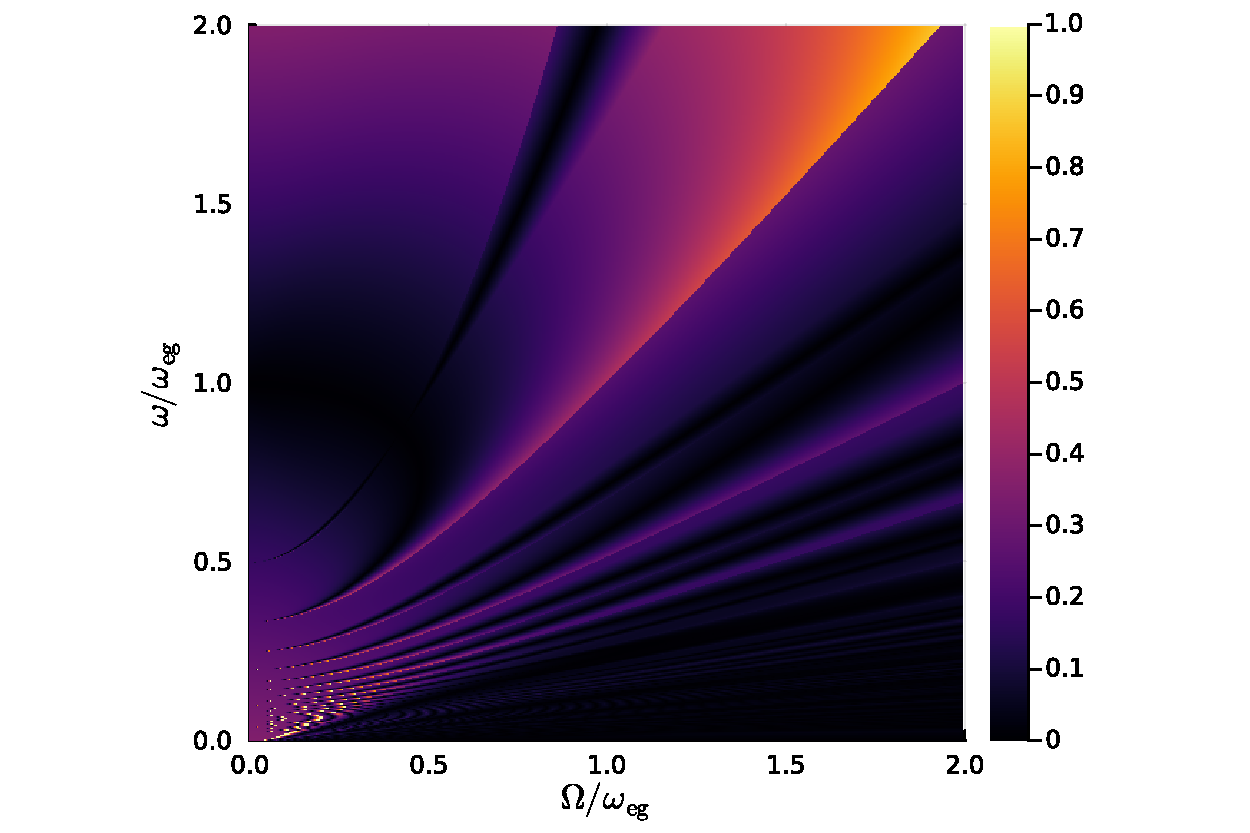
\includegraphics[width=0.5\textwidth]{plot/relative-error-rwa.pdf}
    \caption{Heatmap of relative error of the spectrum given by RWA, 
    compared to the Floquet quasienergies; 
    $m \omega$ displacements have been added to the latter 
    to minimize their differences with the RWA energies.
    The relative errors of the two energy levels are averaged.
    The discontinuities in the heatmap appear because the true value used in 
    evaluating the relative error of an energy level  
    is the $\varepsilon_n + m \hbar \omega$ 
    that is closest to the RWA energy level, 
    and as the parameters change, $m$ demonstrates non-continuous shifts.}
    \label{fig:rwa-floquet}
\end{figure}

The rotational wave approximation (RWA) is also used 
when a periodic pumping is present, 
and it is not a perturbative theory.
Here we show that it can be seen as a degeneracy case of the Floquet formalism.
Let us again work on the two-level atom model.
Turning back to \eqref{eq:floquet-matrix},
we find that when the driving is nearly resonant, 
or in other words when $\omegaeg - \omega$ is small, 
and when $\Omega$ is also small, starting from the $\ket*{\phi_\text{g}^{(0)}}$ state, 
we are essentially confined in the 
$\ket*{\phi_\text{g}^{(0)}}, \ket*{\phi_{\text{e}}^{(1)}}$ subspace: 
since $\Omega$ is small, 
from $\ket*{\phi_\text{g}^{(0)}}$ it is only possible to jump to 
$\ket*{\phi_\text{e}^{(\pm 1)}}$, 
but then the diagonal element in \eqref{eq:floquet-matrix} is $\omegaeg + \omega \gg \abs*{\omegaeg - \omega}$,
and therefore the transition from $\ket*{\phi_\text{g}^{(0)}}$ to $\ket*{\phi_\text{e}^{(-1)}}$
is much weaker than the transition to $\ket*{\phi_\text{e}^{(1)}}$.
The final effective Hamiltonian therefore becomes 
\begin{equation}
    H = \pmqty{
        0 & - \Omega \\ 
        - \Omega & \underbrace{\omegaeg - \omega}_{\eqqcolon \Delta}
    } =  \Delta \dyad{\tilde{\text{e}}} - \Omega \dyad{\tilde{\text{e}}}{{\text{g}}}  + \text{h.c.}, 
\end{equation}
where $\Delta$ is the detuning and the tilde over e means that 
the state is actually time-dependent in the usual basis 
found by diagonalizing the Hamiltonian of the standalone atom; 
the fact that $\ket*{\tilde{e}}$ is time-dependent is reflected by the fact that 
the matrix elements of other operators, most importantly the dipole, 
under $\{\ket*{\text{g}}, \ket*{\tilde{\text{e}}}\}$ are now time-dependent, 
oscillating at the frequency of $\omega$.

Quantitatively, the relative error of energies given by RWA compared to the true Floquet quasienergies 
are plotted in \prettyref{fig:rwa-floquet}; 
Floquet quasienergies that are closest to the RWA values are picked for comparison.
It can be easily observed that RWA indeed works best 
when $\omega$ is not too far from $\omegaeg$ and $\Omega$ is not too large.
These are the usual condition used when deriving RWA.

\section{Floquet effects in photoemission spectroscopy}

In the last section, we have shown the advantages of the Floquet formalism 
in the strong driving regime.
The physical meanings of the quasi-stationary states and quasienergies however remain unclear:
are they simply tools for simplification of calculation, 
or are they comparable to ``real'' energy levels in some aspects?
In this section we discuss the photoemission spectroscopy of a periodically driven electron band system, 
and show that the quasi-stationary states contribute to the 
electron photoemission intensity in a way similar to 
how conventional band states contribute to the electron photoemission intensity.

Ordinary \ac{arpes} spectra can be captured by Fermi golden rule \cite{sobota2021angle}
\begin{equation}
    I(\vb{k}, \omega) \propto \sum_{\vb{k}', c} 
    \abs*{M_{\vb{k} \vb{k}'}^{fc}}^2 \delta(\omega - \epsilon_{c \vb{k}'}) f(\omega),
    \quad M^{fc}_{\vb{k} \vb{k}'} = \mel{f \vb{k}}{H_{\text{dipole}}}{c \vb{k}'},
    \label{eq:spectral-arpes}
\end{equation}
where $(f, \vb{k})$ is the out-coming electron mode, 
$(c, \vb{k}')$ is an electronic mode within the material 
and $f(\omega)$ is the Fermi-Dirac distribution.
When the starting state is non-equilibrium, 
the spectral function should be replaced by the lesser Green function 
and we get \cite{freericks2009theoretical,rustagi2018photoemission,schuler2021theory,chan2023giant} 
\begin{equation}
    I(t, \vb{k}, \omega) \propto - \ii \int_{t_0}^t \dd{t_1} \int_{t_0}^t \dd{t_2} s(t_1) s(t_2) 
    \sum_{c_1, c_2}
    M_{\vb{k} \vb{k}'}^{fc_1} M_{\vb{k} \vb{k}'}^{fc_2 *} 
    G^<_{\vb{k}' c_2 c_1}(t_2, t_1) \ee^{\ii \omega (t_1 - t_2)} ,
    \label{eq:lesser-arpes}
\end{equation}
where $s(t)$ is the envelope of the probe pulse.
When the system indeed stays in equilibrium when probing starts
and hence $c_1$ is bound to be equal to $c_2$, 
and the probe pulse is long enough and 
hence $s(t)$ can be seen as a constant and $t \to \infty$, 
it can be directly verified that \eqref{eq:lesser-arpes} 
reduces to the Fermi golden rule \eqref{eq:spectral-arpes}.
% TODO: I'm not sure about the position of t_1 and t_2; 
% specifically, I need to check whether the form here agrees with the pure 
% obtained in the pure state formalism starting from an eigenstate
When the system is Floquet-driven, this reduction fails, 
and there is no guarantee that $c_2$ equals $c_1$ for non-zero terms;
in other words, there is possible band renormalization in the system.
The $MM^*$ factor can be regarded as a constant for a rough estimation 
\cite{freericks2009theoretical,chan2023giant},
and in the long probe pulse limit, \eqref{eq:lesser-arpes} becomes 
\begin{equation}
    I(t \to \infty, \vb{k}, \omega) \propto
    - \ii \int \dd{\bar{t}} \int \dd{\tau} G^<_{\vb{k}' c_2 c_1}(\bar{t}, \bar{t} + \tau) \ee^{\ii \omega \tau} 
    = - \ii \expval{\int \dd{\tau} \ee^{\ii \omega \tau}
    \sum_{c_1, c_2} G^<_{\vb{k}' c_2 c_1}(\bar{t}, \bar{t} + \tau)}_{\bar{t}},
\end{equation} 
and if the time averaged $G^<$ is diagonalized under the $c$ basis, 
we have arrived at a generalized Fermi golden rule.
We then note that the averaged lesser Green function is indeed diagonalized under the Floquet basis \cite{rudner2020floquet}:
\begin{equation}
    \bar{\rho}_{\vb{k}}(\Omega) = - \ii \expval{\int \dd{\tau} \ee^{\ii \omega \tau} G^<_{\vb{k}}} 
    =\sum_{n \vb{k}, m} A_{n \vb{k}}^{(m)} \delta\left(\varepsilon_{n \vb{k}} +m \omega-\Omega\right), 
    \quad A_{n \vb{k}}^{(m)}= \braket*{\phi_{n \vb{k}}^{(m)}}{\phi_{n \vb{k}}^{(m)}}.
\end{equation}
The ARPES spectrum of a Floquet-driven band structure, therefore, 
is given by all Floquet bands weighted by the magnitude of $\ket*{\phi_{n \vb{k}}^{(m)}}$.

Interestingly, it is possible to use light to stimulate 
some long-lived degrees of freedom in a solid 
and let it drive the rest of the system, 
which sometimes is known as ``self-driving''.
In \cite{chan2023giant}, it is demonstrated that 
Floquet renormalization of the band structure can be observed 
even long after the pump is turned off, 
which is due to the existence of excitons previously created by the pump.
TODO: exciton captured by electron self-energy; 
exciton creates $\Sigma_{cv}$

In principle there are indefinite exciton-driven Floquet quasi-band ARPES signatures,
but since the signatures are weighted by $A^{(m)}_{n \vb{k}}$,
which are usually small when $\abs*{m}$ is large, 
usually only the $m=1$ Floquet signatures are important,
which can be calculated from Fermi golden rule in a more conventional way.


\section{Discussion}

In this report,
we have reviewed the basic theory of Floquet formalism, 
where in a driven system with a $N$-dimensional Hilbert space, 
an arbitrary state can be expanded into 
the linear combination of $N$ quasi-stationary states, 
whose time evolution is directed by quasienergies,
and both the quasi-stationary states and quasienergies can be obtained 
by diagonalizing the Floquet effective Hamiltonian.
We have also compared the Floquet formalism with the two other approaches often used for driving systems, 
namely time-dependent perturbation theory and the rotating wave approximation;
it can be seen that 

Finally, we demonstrate that 

\printbibliography

\end{document}